%!TEX program = xelatex
%Template created by: Maciej Byczko
\documentclass[a4paper,12pt]{extarticle}  %typ dokumentu

\usepackage{geometry} %poprawienie marginesów
\usepackage{polski} %polskie znaki
\usepackage{graphicx} %grafiki
\usepackage{float} %poprawienie pozycji
\usepackage{fancyhdr} % header i footer
\usepackage{hyperref} %tworzenie odnośników, \url{<url>}, \href{<file path, link>}{<text with link>} \pageref{}

\graphicspath{{pictures/}}
\geometry{margin=0.7in}
\pagestyle{fancy}
\cfoot{Strona \thepage}
\rhead{Strona \thepage}
\lhead{\typdoc}
\setlength{\headheight}{15pt}

%Ustawienie paczki hyperref
\hypersetup{
     colorlinks,
     citecolor=black,
     filecolor=black,
     linkcolor=black,
     urlcolor=black
}


\title{\tytul \\ \small{\opis}}
\author{\tworcy}
\date{\data}

%-----------------------SEKCJA DANYCH----------------------------------
\def\tytul{Technologie Sieciowe - Projekt} %<<< tytuł ćwiczenia
\def\nrcw{} %<<< numer ćwiczenia
\def\data{\today \\ \small{\zajinfo}} %<< data wykonania
\def\prowadzacy{Prowadzący: dr. inż Arkadiusz Grzybowski} %<<<prowadzący
\def\nrgrupy{} %<<<numer grupy
\def\tworcy{Autorzy:\\Karol Baraniecki (252726)\\Maciej Byczko(252747)} %<<< autorzy
\def\zajinfo{PN 14:00 TP\\ Politechnika Wrocławska\\Wydział Informatyki i Telekomunikacji} %<<< informacje dotyczące zajęć
\def\typdoc{} %<<< typ dokumentu tj Sprawozdanie, zadania itp. {Matematyka dyskretna/Sprawozdanie z Miernictwa}
\def\opis{\prowadzacy} %<<< opis który będzie umieszczony pod tytułem w Maketitle
%----------------------------------------------------------------------


\begin{document}
\maketitle
\tableofcontents
\cleardoublepage
\section{Wstęp}
Celem projektu jest zaprojektowanie lokalnej sieci komputerowej dla firmy programistycznej znajdującej się we Wrocławiu.
Sieć musi zostać zaprojektowana zgodnie ze sprecyzowanymi wymaganiami firmy oraz uwzględniać jej przyszły rozwój.
\subsection{Kadra firmy}
Personel firmy składa się z następujących użytkowników:
\begin{itemize}
	\item Programiści
	\item Testerzy
	\item Projektanci
	\item Marketing
	\item Księgowość
\end{itemize}
\subsection{Opis siedziby firmy}
Przedsiębiorstwo znajduje się przy ulicy Nowowiejskiej 69\label{address}, składa się z dwóch budynków: dwupiętrowego oraz trzypiętrowego.
% W budynkach znajduje się także odpowiednie wyposażenie (serwery,  drukarki,
% komputery,  kamery  IP,  itp.).
% Firma posiada jeden główny punkt dystrybucyjny (MDF) oraz punkty pośrednie (IDF) w każdym z budynków.
\subsubsection{Lokalizacja firmy na mapie}
\begin{minipage}[c]{0.49\linewidth}
	
	\begin{figure}[H]
		\centering
		\resizebox*{\textwidth}{!}{
			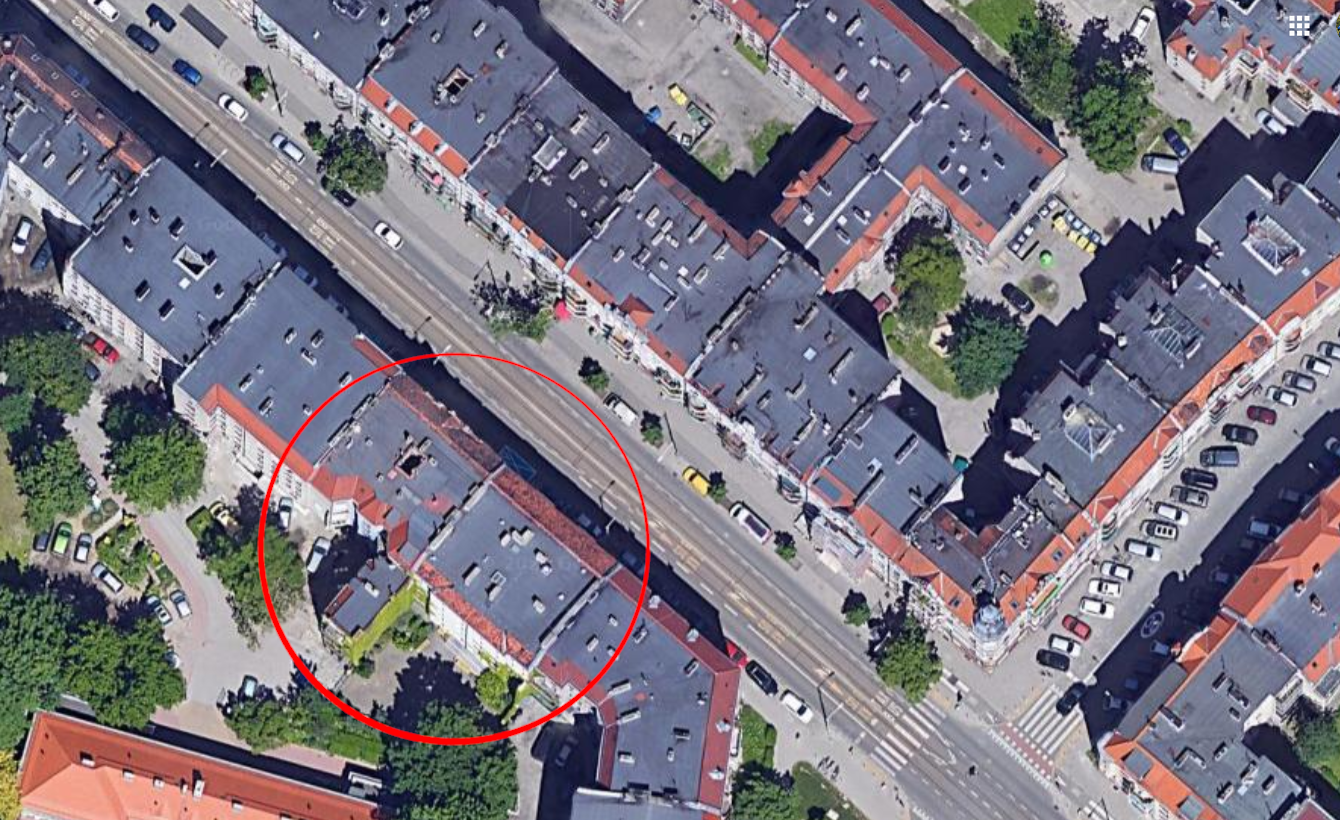
\includegraphics{../pictures/building_close.png}
			}
		\end{figure}
\end{minipage}
\begin{minipage}[c]{0.49\linewidth}
	
	\begin{figure}[H]
		\centering
		\resizebox*{\textwidth}{!}{
			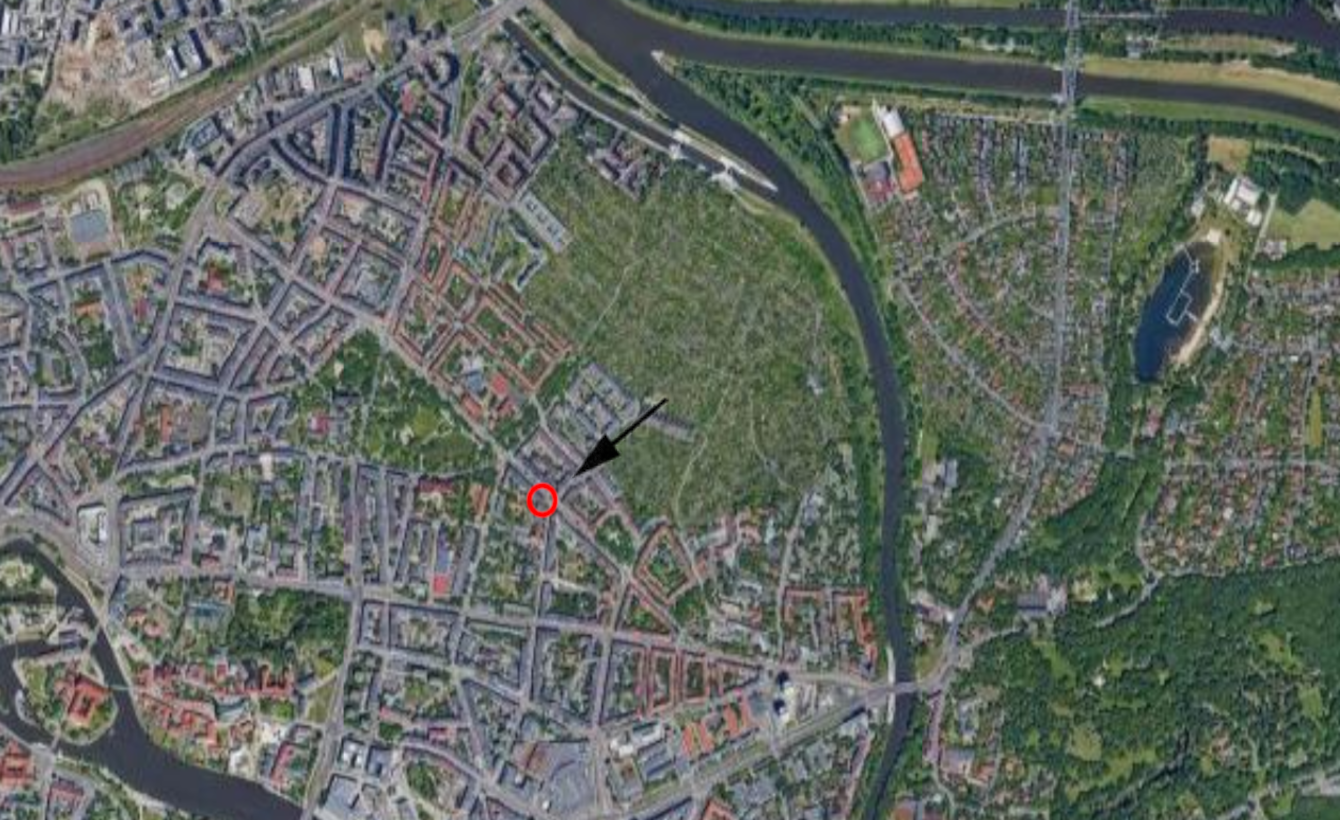
\includegraphics{../pictures/building_not_close.png}
			}
		\end{figure}
\end{minipage}
\subsection{Wymagania}
Firma wymaga od nas aby:
\begin{itemize}
	\item Użyta technologia była z rodziny Ethernet,
	\item na wskazanym piętrze każdego budynku ma być dostępna sieć bezprzewodowa (niezbędna instalacja
	      kablowa jest przygotowana),
	\item należy zapewnić dodatkowe porty na przełącznikach (w liczbie 20\% zajętych portów), w związku z 
	      przewidywanym wzrostem liczby pracowników (w pomieszczeniach są już zainstalowane
	      dodatkowe gniazda sieciowe),
	\item ruch w ramach grup roboczych ma być separowany z wykorzystaniem sieci VLAN,
	\item należy  zapewnić  dwa  podłączenia  do  Internetu:  podstawowe  oraz  zapasowe,  o  przepustowości
	      adekwatnej do potrzeb przedsiębiorstwa,
	\item podstawowe  łącze  internetowe  ma  zapewniać  gwarancję  minimalnej  przepustowości  równej  co
	      najmniej 40\% średniego przewidywanego przepływu na tym łączu, 
	\item kosztorys ma uwzględniać koszt wszystkich urządzeń, podłączenia do Internetu i koszt korzystania z
	      łączy Internetowych w okresie 2 lat
\end{itemize}

\end{document}